%===============================================================================
% Zweck:    KTR-Präsentation-Vorlage
% Erstellt: 15.04.2013
% Autor:    M.G.
%===============================================================================

%===============================================================================
% Zum Kompilieren pdflatex und bibtex ausführen.
%	Konfiguration: in texmaker unter Benutzer -> Benutzerbefehle einen neuen Befehl anlegen: pdflatex -synctex=1 -interaction=nonstopmode %.tex | bibtex % | pdflatex -synctex=1 -interaction=nonstopmode %.tex | pdflatex -synctex=1 -interaction=nonstopmode %.tex
%	Entsprechende Informationen in den config/metainfo verändern
% Zur Auswahl der Sprache im folgenden Befehl
% ngerman für deutsch eintragen, english für Englisch.
%===============================================================================

% Options ngerman, english
\newcommand{\lang}{english}

\documentclass[11pt,\lang ,
%draft,
%handout,
compress
]{beamer}
% Für den Header
% Modify for different languages
\usepackage{ifthen}

\newcommand{\unibastring}{\ifthenelse{\equal{\lang}{ngerman}}{Universit\"at Bamberg}{University of Bamberg}}

\usepackage{etex}
\usepackage{stmaryrd}
\usetheme{UniBa}
%\usefonttheme{
%	default | professionalfonts | serif |
%	structurebold | structureitalicserif |
%	structuresmallcapsserif
%}
\usefonttheme{professionalfonts}
%\useinnertheme{
%	circles | default | inmargin |
%	rectangles | rounded
%}
\useinnertheme{rectangles}
%\useoutertheme{
%	default | infolines | miniframes |
%	shadow | sidebar | smoothbars |
%	smoothtree | split | tree
%}
%\useoutertheme{split}
\setbeamercovered{transparent}

% Without navigation symbols
\beamertemplatenavigationsymbolsempty

%% Formatierungen
\usepackage{url}
\usepackage{latexsym}			% schönere Symbole
\usepackage{color}
%\usepackage{float}

%% Zeichensätze
\usepackage[utf8]{inputenc}
\usepackage[iso]{umlaute}
\usepackage{lmodern}
\usepackage{float}
\usepackage{thumbpdf}
\usepackage{wasysym}
\usepackage{ucs}

%Meta info
%Necessary Information
\author[M. Großmann]{Marcel Großmann}
\title{WebRTC}
\subtitle{The Web Way to Communicate}
%The day of the presentation
\date{4. February 2014}

%Optional Information
\subject{Project}
\keywords{Project, WebRTC, Informatic}

%Already set
\ifthenelse{\equal{\lang}{ngerman}}{%
\institute[KTR]{Professur f\"ur Informatik\\%
        insbesondere Kommunikationsdienste, Telekommunikationsdienste und Rechnernetze}}{%
\institute[KTR]{Professorship for Computer Science,\\%
        Communication Services, Telecommunication Systems\\%
        and Computer Networks}}

\titlegraphic{
\includegraphics[width=13mm,height=13mm]{image/logo}}


%% Hyperref
\usepackage{hyperref}

\makeatletter
\hypersetup{pdftitle={\@title}, pdfauthor={\@author}, linktoc=page, pdfborder={0 0 0 [3 3]}, breaklinks=true, linkbordercolor=unibablueI, menubordercolor=unibablueI, urlbordercolor=unibablueI, citebordercolor=unibablueI, filebordercolor=unibablueI}
\makeatother
%% Define a new 'leo' style for the package that will use a smaller font.
\makeatletter
\def\url@leostyle{%
  \@ifundefined{selectfont}{\def\UrlFont{\sf}}{\def\UrlFont{\small\ttfamily}}}
\makeatother
%% Now actually use the newly defined style.
\urlstyle{leo}

%% Sprache
\ifthenelse{\equal{\lang}{ngerman}}{\usepackage[german,ngerman]{babel}}{\usepackage[\lang]{babel}}
%\mode<presentation>{
%% XXX without this the number does not appear
%\AtBeginDocument{\def\figurename{{\scshape Fig.~\thefigure}}}
%}
%%\usepackage{abstract}

%% Mathe und Formeln
\usepackage{calc}
\usepackage{amsmath}
\usepackage{amssymb,amsthm,amsfonts}
\usepackage{dsfont}
\usepackage[nice]{nicefrac}
\usepackage{cancel}  %%druchstreichen von Formeln
%
%% Programmieren mit Latex
\usepackage{ifthen}


\usepackage{dirtree}   %setzen von baumstrukturen

%%%   Fuer anspruchsvolle Tabellen   %%
\usepackage{longtable, colortbl}
\usepackage{multicol, multirow}
%
%%%  Für Grafiken %%
\usepackage{graphicx}
\usepackage{pdfpages}
\usepackage{tikz}
%\usepackage{pgfplots}
\usetikzlibrary{calc,arrows,fit,positioning,trees,snakes,backgrounds,shadows,decorations,decorations.markings,decorations.shapes,shapes,patterns,fadings}
\usepackage[font=footnotesize]{subfig}

\usepackage[underline=true,rounded corners=false]{pgf-umlsd}
%\usepackage{fp}
%
%%%  Zur Darstellung des Euro-Symbols   %%
%\usepackage{eurosym, wasysym}
%\selectlanguage{german}
%
%%%   Fuer Bibtex nach APA Style (American Psychology Association)   %%
%\usepackage[numbers]{natbib}
\usebibitemtemplate{\insertbiblabel}

%% Code-Hervorhebung
%% Quellcode

%\usepackage[numbered,autolinebreaks,useliterate]{mcode}
%\usepackage{verbatim}            % Quellcode einbinden (\verbatiminput) standardpaket
%\usepackage{moreverb} 
%% PseudoCode
%\usepackage{algorithm}
\usepackage{algpseudocode}
%%\usepackage{algorithmicx}
%%\floatname{algorithm}{Algorithmus}
%\algrenewcommand{\algorithmiccomment}[1]{\hskip1em\textcolor{gray!60}{$\rhd$ #1}}
%%\renewcommand{\listalgorithmname}{Algorithmen}
%%\def\algorithmautorefname{Algorithmus}
%
%%% Code Highlighting
%\definecolor{mygray}{gray}{.75}
\usepackage{listings} 

\lstdefinelanguage{JavaScript}{
  keywords={break, case, catch, continue, debugger, default, delete, do, else, false, finally, for, function, if, in, instanceof, new, null, return, switch, this, throw, true, try, typeof, var, void, while, with},
  morecomment=[l]{//},
  morecomment=[s]{/*}{*/},
  morestring=[b]',
  morestring=[b]",
  ndkeywords={class, export, boolean, throw, implements, import, this},
  keywordstyle=\color{unibablueI},
  ndkeywordstyle=\color{unibagreenI},
  identifierstyle=\color{black},
  commentstyle=\color{unibagrayI}\ttfamily,
  stringstyle=\color{unibaredI}\ttfamily,
  sensitive=true
}

\lstset{
   language=JavaScript,
  % backgroundcolor=\color{lightgray},
   extendedchars=true,
   basicstyle=\footnotesize\ttfamily,
   showstringspaces=false,
   showspaces=false,
   numbers=left,
   numberstyle=\scriptsize,
   numbersep=9pt,
   tabsize=2,
   breaklines=true,
   showtabs=false,
   captionpos=b
}


%\lstset{numbers=left, numberstyle=\tiny, numbersep=6pt} 
\lstset{language=JavaScript}
%\lstset{classoffset=1, morekeywords={mycontext}, keywordstyle=\color{darkgreen}, classoffset=0, keywordstyle=\color{darkblue}}
%\lstset{basicstyle=\small, showstringspaces=false, commentstyle=\color{unibagrayI}, breaklines=true, captionpos=b}
%\renewcommand{\lstlistingname}{Code-Ausschnitt}
%\renewcommand{\lstlistlistingname}{Code-Ausschnitte}
%\def\lstlistingautorefname{Code-Ausschnitt}


%%%%%%%%%%%%%%%%%%%%%%%%%%%%%%%%%%%%%%%%%%%%%%%%%%%%%%%%%%%%%%%%%%%%%%%%%%%%%%%%%%%%%%%%%%%%
%%%                                   COMMAND SETUP                                       %%
%%%%%%%%%%%%%%%%%%%%%%%%%%%%%%%%%%%%%%%%%%%%%%%%%%%%%%%%%%%%%%%%%%%%%%%%%%%%%%%%%%%%%%%%%%%%

%#1 Breite
%#2 Datei (liegt im image Verzeichnis)
%#3 Beschriftung
%#4 Label fuer Referenzierung
\newcommand{\image}[4]{
\begin{figure}[H]
\centering
\includegraphics[width=#1]{image/#2}
\caption{\footnotesize{#3}}
\label{#4}
\end{figure}
}

%#1 Breite
%#2 Datei (liegt im image Verzeichnis)
%#3 Beschriftung
%#4 Label fuer Referenzierung
\newcommand{\pic}[2]{
\begin{figure}[H]
\centering
\includegraphics[width=#1]{image/#2}
\end{figure}
}


% #1 videofile
% #2 scalefactor
\newcommand{\video}[2]{%
\includemovie[text={\includegraphics[scale=#2]{praesi/video/#1.png}}, autoplay, mouse=true, repeat=1]{}{}{praesi/video/#1.swf}}

%% Fancy Quotes
\makeatletter
\tikzset{%
  fancy quotes/.style={
    text width=\fq@width pt,
    align=justify,
    inner sep=1em,
    anchor=north west,
    minimum width=\textwidth,
  },
  fancy quotes width/.initial={.8\textwidth},
  fancy quotes marks/.style={
    scale=8,
    text=white,
    inner sep=0pt,
  },
  fancy quotes opening/.style={
    fancy quotes marks,
  },
  fancy quotes closing/.style={
    fancy quotes marks,
  },
  fancy quotes background/.style={
    show background rectangle,
    inner frame xsep=0pt,
    background rectangle/.style={
      fill=unibagrayIV,
      rounded corners,
    },
  }
}

\newenvironment{fancyquotes}[1][]{%
\noindent
\tikzpicture[fancy quotes background]
\node[fancy quotes opening,anchor=north west] (fq@ul) at (0,0) {``};
\tikz@scan@one@point\pgfutil@firstofone(fq@ul.east)
\pgfmathsetmacro{\fq@width}{\textwidth - 2*\pgf@x}
\node[fancy quotes,#1] (fq@txt) at (fq@ul.north west) \bgroup}
{\egroup;
\node[overlay,fancy quotes closing,anchor=east] at (fq@txt.south east) {''};
\endtikzpicture}

\makeatother

\def\signed #1{{\leavevmode\unskip\nobreak\hfil\penalty50\hskip2em
  \hbox{}\nobreak\hfil(#1)%
  \parfillskip=0pt \finalhyphendemerits=0 \endgraf}}

\newsavebox\mybox
\newenvironment{aquote}[1]
  {\savebox\mybox{#1}\begin{fancyquotes}}
  {\signed{\usebox\mybox}\end{fancyquotes}}



\hyphenation{op-tical net-works semi-conduc-tor}

\setbeamertemplate{caption}[numbered]
%\numberwithin{figure}{section}
\begin{document}

\frame{\titlepage}

\AtBeginSection[]
{
  \frame<handout:0>
  {
    \frametitle{Outline}
    \tableofcontents[currentsection,hideallsubsections]
  }
}

\AtBeginSubsection[]
{
  \frame<handout:0>
  {
    \frametitle{Outline}
    \tableofcontents[sectionstyle=show/hide,subsectionstyle=show/shaded/hide,subsubsectionstyle=hide]
  }
}

%\AtBeginSubsubsection[]
%{
%  \frame<handout:0>
%  {
%    \frametitle{Outline}
%    \tableofcontents[sectionstyle=show/hide,subsectionstyle=show/shaded/hide,subsubsectionstyle=show/shaded/hide]
%  }
%}

\newcommand<>{\highlighton}[1]{%
  \alt#2{\structure{#1}}{{#1}}
}

\newcommand{\icon}[1]{\pgfimage[height=1em]{#1}}



%\section*{}
%\begin{frame}{Content}
%\tableofcontents
%\end{frame}
%%%%%%%%%%%%%%%%%%%%%%%%%%%%%%%%%%%%%%%%%
%%%%%%%%%% Content starts here %%%%%%%%%%
%%%%%%%%%%%%%%%%%%%%%%%%%%%%%%%%%%%%%%%%%
\section*{}
%\nocite*
\begin{frame}{References}
\def\newblock{\hskip .11em plus .33em minus .07em}
\footnotesize
\bibliographystyle{IEEEtran}
\bibliography{literature/bib}
\normalsize
\end{frame}

%\begin{frame}{Online Tutorials}
%\begin{itemize}
%\item \textbf{Android Developers:} \url{http://developer.android.com/guide/index.html}
%\url{http://developer.android.com/resources/tutorials/hello-world.html}
%\item \textbf{AndroidPIT}\\ \url{http://www.androidpit.de/de/android/wiki/view/Android_Anf\%C3\%A4nger_Workshop}
%\item \textbf{Lars Vogel}\\ \url{http://www.vogella.com/articles/Android/article.html}
%\url{http://www.vogella.com/android.html}
%\end{itemize}
%\end{frame}
%
%\begin{frame}{Development Environments}
%\begin{itemize}
%\item \textbf{Java}\\
%\url{http://www.oracle.com/technetwork/java/javase/downloads/index.html}
%\item \textbf{Eclipse}\\
%\url{http://www.eclipse.org/}
%\item \textbf{Android SDK}\\
%\url{http://developer.android.com/sdk/index.html}
%\item \textbf{Android Eclipse Plugin} (Eclipse update site)\\
%\url{https://dl-ssl.google.com/android/eclipse}
%\end{itemize}
%\end{frame}

\begin{frame}{Real-Time Communication on the Internet}

\begin{itemize}
\item NVP (Network Voice Protocol) - 1977
\item RTP (Real-time Transport Protocol) -1992
\begin{itemize}
\item First published as IETF RFC in 1996
\item Still used today for VoIP and with SIP
\end{itemize}
\item ITU H.323 video telephony standard - 1996
\item IETF SIP (Session Initiation Protocol) - 1999
\begin{itemize}
\item Unleashed VoIP revolution on telphony
\item Video and room conferencing
\item Protocol widely used by service providers and in enterprises
\end{itemize}
\item Real-Time Communcation on the Web
\begin{itemize}
\item Voice and video on the Internet using browser plugins
\item 2006 with GoogleTalk inside Gmail
\item WebRTC standardizes and eliminates need for plugin or download
\end{itemize}
\end{itemize}

\end{frame}

\begin{frame}{Why not just use Flash?}
\begin{columns}
\column{.5\textwidth}
\textbf{Pros}
\begin{itemize}
\item Most browser already have Flash plugin
\item Streaming audio and video uses Flash today
\item Flash supports real-time audio and video
\item Web developers familiar with Flash
\end{itemize}
\column{.5\textwidth}
\textbf{Cons}
\begin{itemize}
\item Flash is single-vendor proprietary and closed
\item Losing market share and not available on iOS
\item Limited codec and echo cancellation options
\item Proprietary development tools
\end{itemize}
\end{columns}
\end{frame}

\begin{frame}{WebRTC is ``Skype in the browser''}
\begin{itemize}
\item Access to camera and microphone without a plugin ($\rightarrow$ No more Flash!)
\item Audio/video direct from browser to browser
\item Why does it matter?
\begin{itemize}
\item Media can stay local
\item Mobile devices eventually dropping voice channel anyway
\item Games
\end{itemize}
\end{itemize}
\end{frame}

\begin{frame}{The Browser RTC Function}

\begin{columns}
\column{.5\textwidth}
\begin{itemize}
\item New Browser Real-Time Communication (RTC) Function built-in to browsers
\item Contains
\begin{itemize}
\item Audio and video codecs
\item Ability to negotiate peer-to-peer connections
\item Echo cancellation, packet loss concealment
\end{itemize}
\item In Chrome and Mozilla today
\end{itemize}
\column{.5\textwidth}

\end{columns}

\end{frame}

\begin{frame}{So What's the Big Deal}
\begin{itemize}
\item The web is now a platform for real-time communications development
\item Communication will be secure (encrypted) by default
\item Latest audio and video codecs means superior quality to anything else
\item WebRTC provides peer-to-peer media, even through NATs
\item Standard that can interoperate with existing VoIP, video conferencing, and even PSTN
\end{itemize}
\end{frame}

\begin{frame}{WebRTC Triangle}

\begin{itemize}
\item Both browsers running the smae web application from web server
\item Peer Connection media session is establised between them
\item Signaling is not standardized, could be SIP, Jingle, proprietary. Uses HTTP or WebSockets for transport
\end{itemize}
\end{frame}

\begin{frame}{WebRTC Trapezoid}

\begin{itemize}
\item Similar to SIP Trapezoid
\item Web Servers communicatie using SIP or Jingle
\item Useful for building conventional telephony apps, but unclear how this works in the web world
\end{itemize}
\end{frame}

\begin{frame}{WebRTC and SIP}
\begin{itemize}
\item Peer Connection appears as a standard RTP media session, described by SDP
\item Web Server implements a JSEP (JavaScript Session Establishment Protocol) to SIP signaling gateway
\item SIP Endpoint must support RTCWEB Media extensions (ICE NAT Traversal, Secure RTP, etc.)
\end{itemize}
\end{frame}

\begin{frame}{WebRTC with SIP}
\begin{itemize}
\item Browser runs a SIP User Agent by running JavaScript form Web Server
\item Secure RTP media connection uses WebRTC APIs
\item Details in [draft-ietf-sipcore-websocket] that defines SIP transport over WebSockets
\end{itemize}
\end{frame}

\begin{frame}{WebRTC and PSTN}
\begin{itemize}
\item Peer Connection terminates ona PSTN Gateway
\item Audio only
\item Could also use SIP trunking such as SIPconnect 1.1 recommendation
\end{itemize}
\end{frame}

\begin{frame}{WebRTC Support fo Multiple Media}
\begin{itemize}
\item Multiple sources of audio and video are assumed and supported
\item All RTP media, voice and video, and RTCP feedback messages are multiplexed over the same UDP port and address
\end{itemize}
\end{frame}

\begin{frame}{How to use WebRTC}
\begin{tikzpicture}
\node at (0,0) {\includegraphics[page=9,height=\textheight]{image/webrtc.pdf}};
\node[align=center, nounibaredII] at (4.5,1) {A few lines of\\ JavaScript is all\\ that is needed!};
\end{tikzpicture}
\end{frame}

\begin{frame}{WebRTC Peer-to-Peer Media}\framesubtitle{Media Flows in WebRTC}
\begin{figure}
\includegraphics[page=10,width=\textwidth]{image/webrtc.pdf}
\end{figure}
\end{frame}

\begin{frame}{WebRTC Peer-to-Peer Media}\framesubtitle{Media without WebRTC}
\begin{tikzpicture}
\node at (0,0) {\includegraphics[page=11,width=\textwidth]{image/webrtc.pdf}};
\node[align=center, nounibaredII] at (-3,-3) {A browser plug-in must be used};
\end{tikzpicture}
\end{frame}

\begin{frame}{WebRTC Peer-to-Peer Media}\framesubtitle{Peer-to-Peer Media with WebRTC}
\begin{tikzpicture}
\node at (0,0) {\includegraphics[page=12,width=\textwidth]{image/webrtc.pdf}};
\node[align=center, nounibaredII] at (-3,-3) {No plug-in or download required!};
\end{tikzpicture}
\end{frame}

\begin{frame}{WebRTC Peer-to-Peer Media}\framesubtitle{NAT Complicates Peer-to-Peer Media}
\begin{tikzpicture}
\node at (0,0) {\includegraphics[page=13,width=\textwidth]{image/webrtc.pdf}};
\node[align=center, nounibaredII, font=\footnotesize] at (3.5,-3.5) {Most browsers are behind NATs\\ on the Internet, which\\ complicates the establishment\\ of peer-to-peer media sessions};
\node[align=center, nounibaredII] at (-3,-3) {Network Address Translator};
\end{tikzpicture}
\end{frame}

\begin{frame}{WebRTC Peer-to-Peer Media}\framesubtitle{NAT Media Through NAT}
\begin{tikzpicture}
\node at (0,0) {\includegraphics[page=14,width=\textwidth]{image/webrtc.pdf}};
\node[align=center, nounibaredII, font=\footnotesize] at (3.5,-3.5) {ICE hole punching can often\\ establish a direct peer-to-peer\\ session between browsers\\ behind different NATs};
\node[align=center, nounibaredII] at (-3,-3) {Interactive Communications\\ Establishment, RFC 5245};
\end{tikzpicture}
\end{frame}

\begin{frame}{WebRTC Peer-to-Peer Media}\framesubtitle{P2P Media Can Stay Local to NAT}
\begin{tikzpicture}
\node at (0,0) {\includegraphics[page=15,width=\textwidth]{image/webrtc.pdf}};
\node[align=center, nounibaredII, font=\footnotesize] at (3.5,-3.5) {If both browsers are behind the\\ same NAT, hole punching can\\ often establish a connection\\ that never leaves the NAT};
\end{tikzpicture}
\end{frame}

\begin{frame}{WebRTC Peer-to-Peer Media}\framesubtitle{Browser Queries STUN Server}
\begin{tikzpicture}
\node at (0,0) {\includegraphics[page=16,width=\textwidth]{image/webrtc.pdf}};
\node[align=center, nounibaredII, font=\footnotesize] at (3.5,-3.5) {Browser sends STUN test\\ packet to STUN server to\\ learn its public IP address\\ (address of the NAT)};
\node[align=center, nounibaredII] at (-3,-3) {Session Traversal Utilities\\ for NAT, RFC 5389};
\end{tikzpicture}
\end{frame}

\begin{frame}{WebRTC Peer-to-Peer Media}\framesubtitle{TURN Server Can Relay Media}
\begin{tikzpicture}
\node at (0,0) {\includegraphics[page=17,width=\textwidth]{image/webrtc.pdf}};
\node[align=center, nounibaredII, font=\footnotesize] at (3.5,-3.5) {In some cases, hole punching\\ fails, and a TURN Media Relay\\ on the public Internet must be used.};
\node[align=center, nounibaredII] at (-3,-3) {Traversal of UDP\\ aRound NAT, RFC 5766};
\end{tikzpicture}
\end{frame}


%%%%%%%%%%%%%%%%%%%%%%%%%%%%%%%%%%%%%%%%%
%%%%%%%%%% References          %%%%%%%%%%
%%%%%%%%%%%%%%%%%%%%%%%%%%%%%%%%%%%%%%%%%
%\section*{}
%\begin{frame}[allowframebreaks]{References}
%\def\newblock{\hskip .11em plus .33em minus .07em}
%\scriptsize
%\bibliographystyle{IEEEtran}
%\bibliography{literature/bib}
%\normalsize
%\end{frame}
%



%% Last frame
\frame{
  \vspace{2cm}
  {\huge Questions ?}

  \vspace{20mm}
  \nocite*
  
  \begin{flushright}  
    Marcel Gro\ss mann
    
    \structure{\footnotesize{\href{mailto:marcel.grossmann@uni-bamberg.de}{marcel.grossmann@uni-bamberg.de}}}
  \end{flushright}
}


\end{document}
